\input{styleDS}
\usepackage{enumitem}
\def\numero{Révisions 4}
\def\classe{Option info MP1}
\renewcommand*{\arraystretch}{1.2}
\usetikzlibrary[automata]
\setcounter{secnumdepth}{3}
\renewcommand{\thesection}{\Roman{section}}
\renewcommand{\thesubsection}{\thesection.\Alph{subsection}}
\renewcommand{\thesubsubsection}{\thesection.\Alph{subsection}.\arabic{subsubsection})}
\camltrue
%-------------------------------------------------------------------------------
%-------------------------------------------------------------------------------
%-------------------------------------------------------------------------------
\begin{document}
%-------------------------------------------------------------------------------
%-------------------------------------------------------------------------------
%-------------------------------------------------------------------------------
\chapter{Mots synchronisants, Centrale 2017}
%-------------------------------------------------------------------------------
%-------------------------------------------------------------------------------
%-------------------------------------------------------------------------------
\section{Considérations générales}
%-------------------------------------------------------------------------------
%-------------------------------------------------------------------------------
%--------------------   I.A   --------------------------------------------------
%-------------------------------------------------------------------------------
\subsection{}Dans une machine à un seul état tout mot envoie cet état dans lui-même donc est synchronisant.

%--------------------   I.B   --------------------------------------------------
%-------------------------------------------------------------------------------
\subsection{}
Dans $M_1$ les états $1.a^n=1\ne 2=2.a^n$ si $n$ est pair et $1.a^n=2\ne 1=2.a^n$ si $n$ est impair donc aucun mot sur $\{a\}$ ne synchronise $M_1$.
%--------------------   I.C   --------------------------------------------------
%-------------------------------------------------------------------------------
\subsection{}
$ada$, entre autres, est synchronisant.
%--------------------   I.D   --------------------------------------------------
%-------------------------------------------------------------------------------
\subsection{}
\begin{lstlisting}
let rec delta_etoile mch etat mot =
  match mot with
  |[] -> etat
  |x::u -> delta_etoile mch (mch.delta etat x) u;;
\end{lstlisting}
%--------------------   I.E   --------------------------------------------------
%-------------------------------------------------------------------------------
\subsection{}
\begin{lstlisting}
let est_synchronisant mch mot =
  let n = mch.n_etats in  
  let fin = delta_etoile mch 0 mot in
  let i = ref 1 in
  while !i < n &&  (delta_etoile mch !i mot = fin)
    do i := !i + 1 done;
  i = n;;
\end{lstlisting}
%--------------------   I.F   --------------------------------------------------
%-------------------------------------------------------------------------------
\subsection{}
Pour tout mot $u$ on note $f_u$ la fonction de $Q$ dans $Q$ qui associe $q.u$ à $q$.

Si $u = x_1x_2\cdots x_p$ alors $f_u = f_{x_p}\circ \cdots \circ f_{x_1}$.
 
L'existence d'un mot synchronisant implique l'existence d'un mot $u$ tel que $f_u$ n'est pas surjective car son image est réduite à un état et $Q$ contient au moins deux état. Parmi les lettres de $u$ il en existe au moins une, $y$, telle que $f_y$ n'est pas bijective car sinon $f_u$ le serait.

Comme $Q$ est fini, $f_y$ non bijective ne peut être injective donc 

il existe $q\ne q'$ tels que $f_y(q)=q.y \ne f_y(q') = q'.y$.
%--------------------   I.G   --------------------------------------------------
%-------------------------------------------------------------------------------
\subsection{Machine des parties}
%--------------------   I.G.1)--------------------------------------------------
%-------------------------------------------------------------------------------
\subsubsection{}
$u$ est synchronisant si et seulement si $\bigl(\hat \delta\bigr)^*(Q, u)$ est un singleton. $M$ admet donc un mot synchronisant si et seulement si un singleton est accessible depuis l'état $Q$.
%--------------------   I.G.2)--------------------------------------------------
%-------------------------------------------------------------------------------
\subsubsection{}
 $LS(M)$ est donc reconnaissable car c'est l'ensemble des mot reconnus par l'automate
$(\widehat Q,\Sigma,\hat \delta,Q,Q_1)$ où $Q_1$ est l'ensemble des singletons de $Q$.
%--------------------   I.G.3)--------------------------------------------------
%-------------------------------------------------------------------------------
\subsubsection{}
L'automate des parties utile depuis $\{0,1,2\}$ s'écrit
%--------------------------------------------------------------------------
\begin{center}
\begin{tabular}{c|cccccc}
& $\{0,1,2\}$ & $\{0,1\}$ & $\{1,2\}$ & $\{0\}$ & $\{1\}$ & $\{2\}$\\
\hline
0 & $\{0,1\}$ & $\{0,1\}$  & $\{0\}$ & $\{1\}$ & $\{0\}$ & $\{0\}$\\
1 & $\{1,2\}$ & $\{1,2\}$  & $\{2\}$ & $\{1\}$ & $\{2\}$ & $\{2\}$\\
\end{tabular}
\end{center}
%--------------------------------------------------------------------------
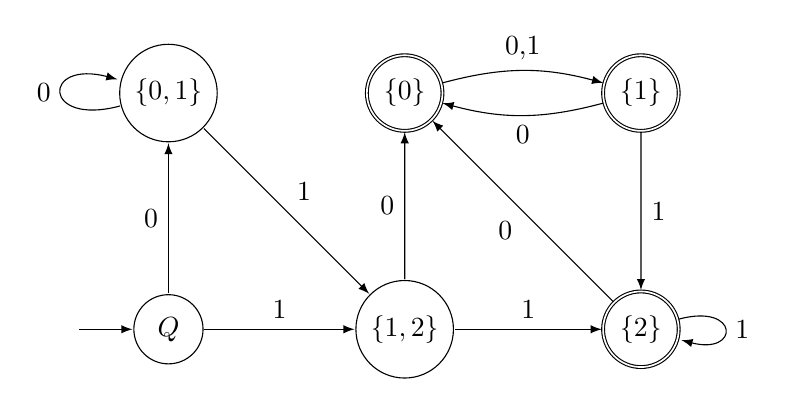
\begin{tikzpicture}[->,auto,>=latex,accepting=accepting by gdouble,
                 initial text =,scale = 1.5]
\node[state,initial]   (N012) at (0,0) {$Q$};
\node[state]           (N12)  at (2,0) {$\{1,2\}$};
\node[state]           (N01)  at (0,2) {$\{0,1\}$};	 
\node[state,accepting] (N0)   at (2,2) {$\{0\}$};	 
\node[state,accepting] (N1)   at (4,2) {$\{1\}$};	 
\node[state,accepting] (N2)   at (4,0) {$\{2\}$};	 
\path (N012) edge                node {1}   (N12)	
             edge                node {0}   (N01)	
       (N01) edge [loop left]    node {0}   (N01)	
             edge                node {1}   (N12)	
       (N12) edge                node {0}   (N0)	
             edge                node {1}   (N2)	
        (N0) edge [bend left=15] node {0,1} (N1)
        (N1) edge                node {1}   (N2)	
             edge [bend left=15] node {0}   (N0)
        (N2) edge [loop right]   node {1}   (N2)	
             edge                node {0}   (N0);
\end{tikzpicture}

Les mots reconnus forment donc le langage dénoté par
\type{(0.0*.1+1).(0+1).(0+1)*}.% ou $0*.1.(0+1).(0+1)*$.
%--------------------   I.H   --------------------------------------------------
%-------------------------------------------------------------------------------
\subsection{}
On transforme $M$ en une machine $M'$ en remplaçant toutes les transitions d'origine $q_0$ en boucles de $q_0$ vers $q_0$ : $q_0$ devient un état-puits.

$q.u$ passe par $q_0$ dans $M$ si et seulement si $q.u$ aboutit à $q_0$ dans $M'$. Ainsi $q.u$ passe par $q_0$ dans $M$ pour tout $q$ implique que $u$ est synchronisant dans $M'$.

Inversement si $u$ est synchronisant dans $M'$ on a $q.u=q_1$ dans $M'$ avec $q_1$ indépendant de $q$. Mais on a toujours $q_0.u=q_0$ donc $q_1=q_0$ : un mot synchronisant dans $M'$ aboutit à $q_0$.

On a ainsi ramené le problème à la recherche d'un mot synchronisant.
%-------------------------------------------------------------------------------
%-------------------------------------------------------------------------------
%-------------------------------------------------------------------------------
\section{Algorithmes classiques}
%-------------------------------------------------------------------------------
%-------------------------------------------------------------------------------
%--------------------  II.A   --------------------------------------------------
%-------------------------------------------------------------------------------
\subsection{Fonctions de files}
La file est remplie quand la fin rejoint le début ; c'est aussi le cas quand la file est vide. C'est pour cette raison qu'il y a un élément qui indique que la file est vide.
%--------------------  II.A.1)--------------------------------------------------
%-------------------------------------------------------------------------------
\subsubsection{}
\begin{lstlisting}
let ajoute f x =
  if f.fin = f.deb && not f.vide
  then failwith "La file est pleine"
  else begin let n = vect_length f.tab in
       f.tab.(f.fin) <- x;
       f.fin <- (f.fin + 1) mod n;
       f.vide <- false end;;
\end{lstlisting}
%--------------------  II.A.2)--------------------------------------------------
%-------------------------------------------------------------------------------
\subsubsection{}
\begin{lstlisting}
let retire f =
  if f.vide
  then failwith "La file est vide"
  else begin let n = vect_length f.tab in
       let y  = f.tab.(f.deb) in
       f.deb <- (f.deb + 1) mod n;
       if f.deb = f.fin then f.vide <- true;
       y end;;
\end{lstlisting}
%--------------------  II.A.3)--------------------------------------------------
%-------------------------------------------------------------------------------
\subsubsection{}
Les deux fonctions ont une complexité constante, ${\cal O}(1)$.
%--------------------  II.B   --------------------------------------------------
%-------------------------------------------------------------------------------
\subsection{}
Dans le programme 1, la première boucle a une longueur déterminée, elle termine.

On ne met dans la file que les sommets tels que $D[s] = \infty$ et on modifie alors la valeurs de $D[s]$ : on ne devra  insérer et extraire de la liste que $|S|$ sommets au plus.

Pour chacun de ces sommets extraites on parcourt leur liste de voisins donc on déterminera le résultat du test $D[s'] = \infty$ au plus $|A|$ fois.

Ainsi l'algorithme termine.
%--------------------  II.C   --------------------------------------------------
%-------------------------------------------------------------------------------
\subsection{}
Comme les opérations du programme se font en temps constant, les arguments ci-dessus montrent que la complexité est en ${\cal O}(|S|+|A|)$.
%--------------------  II.D   --------------------------------------------------
%-------------------------------------------------------------------------------
\subsection{}
On montre que la propriété suivante est un invariant de boucle.


{\it Au début de chaque passage dans la boucle avec une file non vide, en notant  $s_1,s_2,\ldots,s_r$ les éléments de la file par ordre de sortie, il existe un entier $p$ et un indice $k$ vérifiant 

$1\le k\le r$ et $D[s_1] = D[s_2]= \cdots= D[s_k]=p$ et $D[s_{k+1}] = \cdots= D[s_r]=p+1$}

\begin{itemize}
  \item Avant le premier passage dans la boucle {\bf tant que} tous les éléments de la files sont les sommets de $E$ et vérifient $D[s]=0$ : la propriété est vraie initialement avec $p=0$ et $r=k=|E|$.

  \item Si elle est vrai avant un passage on enlève un élément de la file, sa valeur pour $D$ est $p$. 
  
  On ajoute alors les voisins non visités dans la file avec $p+1$ comme valeur de $D$.

On revient alors avant la boucle {\bf tant que} 
\begin{itemize}
    \item Si la file est vide, on finit l'algorithme.
\item Si on avait $k>1$ la propriété est vérifiée avec $k$ diminué de 1 et $p$ inchangé, 
\item Si on avait $k=1$ alors soit la file est vide, soit elle ne contient que des sommets de valeur $p+1$ pour $D$, la propriété est encore vérifiée avec $p$ remplacé par $p+1$ et $k$ égal au nombre d'éléments dans la file.
\end{itemize}
\end{itemize}
%--------------------  II.E   --------------------------------------------------
%-------------------------------------------------------------------------------
\subsection{Calcul de la distance}
%--------------------  II.E.1)--------------------------------------------------
%-------------------------------------------------------------------------------
\subsubsection{}
Chaque sommet dans la file est soit un élément de $E$ soit a été ajouté depuis un élément qui a été dans la file : on en déduit par récurrence sur le rang de sortie que tous les sommets visités sont accessibles depuis $E$.

Inversement si $s$ est un sommet accessible depuis $E$, il existe un chemin 
\[s_0 \rightarrow -> s_1 \rightarrow \cdots \rightarrow -> s_k = s\hbox{ avec }s_0\in E\]

$s_0$ a été ajouté dans la file donc visité et, par récurrence sur $i$, tout sommet du chemin est voisin du sommet précédent dans le chemin donc a été ajouté, soit lors du traitement de $s_{i-1}$, soit auparavant (dans ce cas sa distance a déjà est marque avec une valeur non infinie). En particulier $s$ a été visité.

Ainsi les sommets visités sont tous les sommets accessibles depuis les sommets de $E$ et uniquement ceux-là. Or $D[s] \ne \infty$ si et seulement si $s$ a été visité donc si et seulement si $s$ est accessible depuis un sommet de $E$.

\medskip

$c$ est ainsi le nombre de sommets non accessibles depuis $E$.

De plus, la valeur de $D[s]$, pour $s$ accessible mais n'appartenant pas à $E$, vérifie $D[s] = D[s']+1$ quand il existe une arête de $s'$ à $s$. $D[s]$ est donc la longueur d'un chemin depuis un élément de $E$ vers $s$, elle est donc minorée par la distance minimale : $D[s] \ge d_s$.
%--------------------  II.E.2)--------------------------------------------------
%-------------------------------------------------------------------------------
\subsubsection{}
On considère un chemin de longueur minimale de $s_0\in E$ vers $s$ :

$s_0 \rightarrow s_1 \rightarrow s_2 \rightarrow \cdots \rightarrow s_{p-1} \rightarrow s_p=s$.
En raison de la minimalité on a $d_{s_k} = k$.

$s_{k+1}$ est un voisin de $s_k$ donc il a est marqué (dans $D$) au plus tard lors la lecture de $s_k$ dans la file. En raison de la croissance de la lecture des valeurs de $D[s]$ on en déduit que $D[s_{k+1}]\le D[s_k]+1$.

On a donc $D[s]=D[s_p] \le D[s_0]+p=p=d_s$.

Combinée avec $D[s]\ge d_s$ vue ci-dessus cette inégalité donne $D[s]= d_s$ pour tout sommet accessible ; si $s$ n'est pas accessible on a vu que $D[s]= \infty = d_s$.

Le chemin qui permet d'arriver à $s$ dans l'algorithme est donc un chemin minimal et $P[s]$ indique donc un prédécesseur de $s$ dans ce chemin (avec l'étiquette de la transition).
%--------------------  II.F   --------------------------------------------------
%-------------------------------------------------------------------------------
\subsection{}
On transcrit le pseudo-code.

\type{infini}, \type{rien} et \type{vide} ont été définies globalement.
\begin{lstlisting}
let infini = -1;; 
let vide = (-2, -1);; 
let rien = (-1, -1);;
\end{lstlisting}
On traduit alors presque mot-à-mot le pseudo langage, la seule modification est le traitement du 

{\bf pour tout} $x\in E$ {\bf tel que} condition {\bf faire}

que l'on transforme une une fonction de paramètre \type{list} appelée sur la liste à traiter.
\newpage

\begin{lstlisting}
let accessibles v ens  =
  let n = vect_length v in
  let tableau = Array.make matrix n n 0 in
  let f = {tab = tableau; deb = 0; fin = 0; vide = true} in
  let d = make_vect n infini in
  let p = make_vect n vide in
  let c = ref n in
  let rec init liste = 
    match liste with
    |[] -> ()
    |s::q -> ajoute f s;
             d.(s) <- 0;
             p.(s) <- rien;
             incr c;
             init q in
  init ens;
  let rec traiter s liste =
    match liste with
    |[] -> ()
    |(s1, y)::reste when d.(s1) = infini
                    -> d.(s1) <- d.(s) + 1;
                       p.(s1) <- (s, y);
                       ajoute f s1;
                       c := !c - 1;
                       traiter s reste
    | _::reste -> traiter s reste in 
  while not f.vide do
    let s = retire f in traiter s v.(s) done;
  !c, d, p;;
\end{lstlisting}
%--------------------  II.G   --------------------------------------------------
%-------------------------------------------------------------------------------
\subsection{}
Comme on détermine le sommet depuis la fin, on utilise une fonction récursive terminale. 

On pouvait aussi inverser le résultat d'une fonction récursive non terminale.
\begin{lstlisting}
let chemin s p =
  if p.(s) =  vide
  then failwith "Le sommet n'est pas accessible"
  else let rec construire sommet mot =
         if p.(sommet) = rien  then mot
         else let (prec,y) = p.(sommet) in
              construire prec (y::mot) in
       construire s [];;

\end{lstlisting}
%-------------------------------------------------------------------------------
%-------------------------------------------------------------------------------
%-------------------------------------------------------------------------------
\section{Réduction SAT}
%-------------------------------------------------------------------------------
%-------------------------------------------------------------------------------
%-------------------- III.A   --------------------------------------------------
%-------------------------------------------------------------------------------
\subsection{}
16 sommets \dots
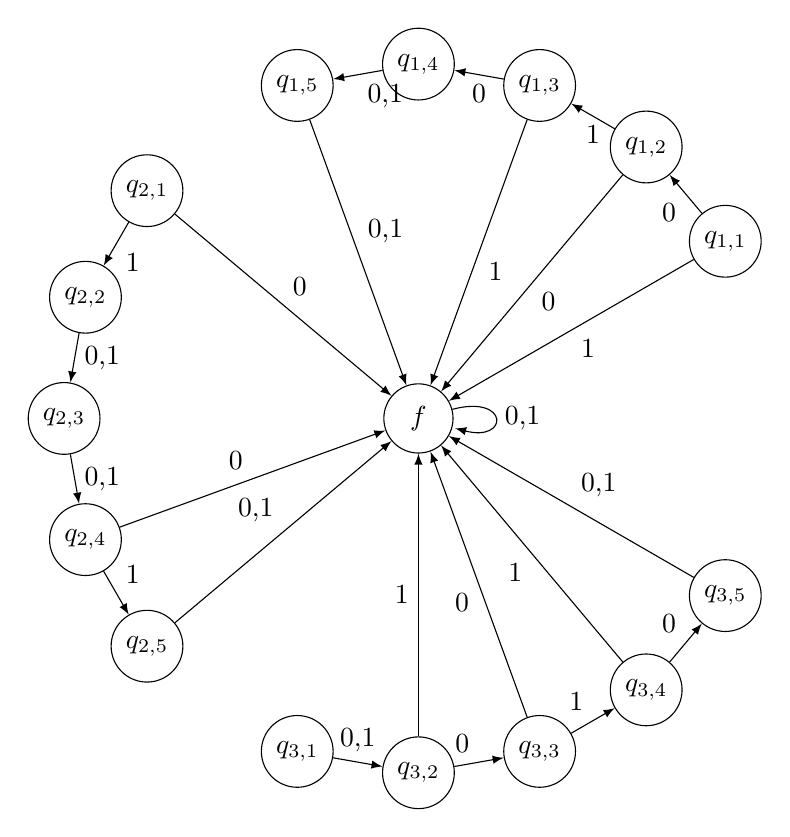
\begin{tikzpicture}[->,auto,>=latex,scale = 1.5]
\node[state] (N11) at (30:3)  {$q_{1,1}$};
\node[state] (N12) at (50:3)  {$q_{1,2}$};
\node[state] (N13) at (70:3)  {$q_{1,3}$};	 
\node[state] (N14) at (90:3)  {$q_{1,4}$};	 
\node[state] (N15) at (110:3) {$q_{1,5}$};	 
\node[state] (N21) at (140:3) {$q_{2,1}$};
\node[state] (N22) at (160:3) {$q_{2,2}$};
\node[state] (N23) at (180:3) {$q_{2,3}$};	 
\node[state] (N24) at (200:3) {$q_{2,4}$};	 
\node[state] (N25) at (220:3) {$q_{2,5}$};	 
\node[state] (N31) at (250:3) {$q_{3,1}$};
\node[state] (N32) at (270:3) {$q_{3,2}$};
\node[state] (N33) at (290:3) {$q_{3,3}$};	 
\node[state] (N34) at (310:3) {$q_{3,4}$};	 
\node[state] (N35) at (330:3) {$q_{3,5}$};	 
\node[state] (F)   at (0:0)   {$f$};	 
\path (N11) edge node {0} (N12)	
            edge node {1} (F)	
      (N12) edge node {0} (F)	
            edge node[below] {1} (N13)	
      (N13) edge node[below] {0} (N14)	
            edge node {1} (F)	
      (N14) edge node[below right] {0,1} (N15)	
      (N15) edge node {0,1} (F);
\path (N21) edge node {0} (F)
            edge node {1} (N22)	
      (N22) edge node[right] {0,1} (N23)	
      (N23) edge node[right] {0,1} (N24)	
      (N24) edge node {0} (F)	
            edge node {1} (N25)	
      (N25) edge node {0,1} (F)	
      (N31) edge node[above] {0,1} (N32)	
      (N32) edge node {0} (N33)	
            edge node {1} (F)	
      (N33) edge node {0} (F)	
            edge node {1} (N34)	
      (N34) edge node {0} (N35)	
            edge node {1} (F)	
      (N35) edge node[above right] {0,1} (F)	
      (F)   edge [loop right] node {0,1} (F);
\end{tikzpicture}
%-------------------- III.B   --------------------------------------------------
%-------------------------------------------------------------------------------
\subsection{}
$(0 ,0 ,0,0)$ est une valuation qui satisfait $F_1$ et \type{0000} est un mot synchronisant.
%-------------------- III.C   --------------------------------------------------
%-------------------------------------------------------------------------------
\subsection{}
Chaque lettre envoie $q_{i,j}$ vers $f$ ou, pour $j\le m$, vers $q_{i,j+1}$ et $f$ est stable par tout mot.

\begin{itemize}
\item Tout mot de longueur 1 envoie $q_{i,m+1}$ vers $f$. On en déduit que tout mot de longueur 1 ou plus envoie $q_{i,m+1}$ vers $f$.

\item Tout mot de longueur 1 envoie $q_{i,m}$ vers $f$ ou $q_{i,m+1}$. Ainsi tout mot de longueur 2 ou plus envoie $q_{i,m}$ vers $f$.

\item Tout mot de longueur 1 envoie $q_{i,m-1}$ vers $f$ ou $q_{i,m}$. D'où tout mot de longueur 3 ou plus envoie $q_{i,m-1}$ vers $f$.

\item On poursuit jusqu'à $q_{i,1}$ qui est envoyé vers $f$ par tout mot de longueur $m+1$ ou plus. 
\end{itemize}
Ainsi tout mot de longueur $m+1$ ou plus est synchronisant.
%-------------------- III.D   --------------------------------------------------
%-------------------------------------------------------------------------------
\subsection{}
On suppose que $F$ est satisfiable par une valuation $(v_1,v_2,\ldots,v_m)$. On considère le mot $u=v_1v_2\cdots v_m$. Comme $u$ est de longueur $m$ on a, d'après la question précédente, $q_{i,k}.u =f$ pour $k\ge 2$. On a aussi $f.u=f$.

Il reste seulement à prouver que $q_{i,1}.u =f$.

Pour chaque clause $C_i$, il existe un littéral $l_k$ tel que sa valeur soit {\bf Vrai} pour la valuation, ce qui signifie que $l_k=x_k$ et $v_k=1$ ou $l_k=\overline{x_k}$ et $v_k=0$.

On suppose que $k_0$ est le plus petit entier vérifiant cette propriété pour la clause $C_i$.

On a alors $q_{i,k_0}.v_{k_0}=f$ et, pour $k < k_0$,

\begin{itemize}
  \item $\overline{x_k}$ n'apparaît pas dans la clause $C_i$ si $v_k=0$ 
  \item ou $x_k$ n'apparaît pas dans la clause $C_i$ si $v_k=1$, 
  \item dans les deux cas  $q_{i,k}.v_k = q_{i,k+1}$.
\end{itemize}
On peut donc calculer le chemin d'étiquette $u$ depuis $q_{i,1}$ :

$q_{i,1}.u = q_{i,1}.v_1v_2\cdots v_m= q_{i,2}.v_2\cdots v_m=
\cdots = q_{i,k_0}.v_{k_0}.v_{k_0+1}\cdots v_m = f.v_{k_0+1}\cdots v_m=f$.

Ainsi $q.u=f$ pour tout état $q$.

Tout mot associé à une valuation qui satisfait la formule est synchronisant.
%-------------------- III.E   --------------------------------------------------
%-------------------------------------------------------------------------------
\subsection{}
Inversement si $u$ est synchronisant pour l'automate avec $|u|\le m$ alors, comme $f.u=f$, on doit avoir $q_{i,1}.u = f$ pour tout $i$. Cela implique qu'il existe un entier $k$ tel que $q_{i,k}.v_k = f$ donc que la valuation associée à $u$ satisfait toutes les clauses donc satisfait la formule. Si le mot est de longueur strictement inférieure à $m$ la valuation est prolongée de manière arbitraire pour les dernières variables.
%-------------------------------------------------------------------------------
%-------------------------------------------------------------------------------
%-------------------------------------------------------------------------------
\section{Existence}
%-------------------------------------------------------------------------------
%-------------------------------------------------------------------------------
%--------------------  IV.A   --------------------------------------------------
%-------------------------------------------------------------------------------
\subsection{Non injectivité}
%--------------------  IV.A.1)--------------------------------------------------
%-------------------------------------------------------------------------------
\subsubsection{}
De manière générale, comme l'automate est déterministe $|E.x| \le |E|$ pour tout ensemble de sommet $E$ et pour toute lettre $x$. On en déduit que $|Q.u_i|$ est décroissante avec, comme $u_r=u$ est synchronisant, $|Q.u_r|=1$.
%--------------------  IV.A.2)--------------------------------------------------
%-------------------------------------------------------------------------------
\subsubsection{}\label{ques:carac}
S'il existe un mot synchronisant $u$ alors $q.u = q'.u$ pour tous états $q$ et $q'$.

\medskip

Inversement on suppose que, pour tout couple d'états $(q,q')$ il existe un mot $u_{q,q'}$ tel que $q.u_{q,q'}=q'.u_{q,q'}$.

On montre alors par récurrence sur $k=|E|$ qu'il existe un mot $u_E$ tel que $|E.u_E| = 1$ pour toute partie $E$ de $Q$.
On dit que $E$ est {\bf synchronisable}.

Pour $|E|=1$ tout mot convient.

On suppose que tout ensemble de cardinal au plus $k$ est synchronisable avec $1\le k < m$.

Si $E$ est de cardinal $k+1$ il a deux élément distincts $q_1$ et $q_2$. On considère $u_1$ tel que $q_1.u_1=q_2.u_1$. L'ensemble $E'=E.u_1$ est donc de cardinal $k$ au plus donc il existe un mot $u_{E'}$ tel que $E'.u_{E'}$ est un singleton par hypothèse de récurrence. 

On a alors 
$E.(u_1.u_{E'}) = (E.u_1).u_{E'} = E'.u_{E'}$ singleton  donc on peut choisir $u_E = u_1.u_{E'}$.

On a alors, pour tout $q\in E$, $q.u_1u_2=q'.u_2=q_0$ car $q'=q.u_1\in E'$ : $E$ est synchronisable.

Tout ensemble de cardinal au plus $k+1$ est synchronisable.

La récurrence est prouvée.

En particulier $Q$ est synchronisable donc $u_Q$ est un mot synchronisant.
%--------------------  IV.B   --------------------------------------------------
%-------------------------------------------------------------------------------
\subsection{}
$|\widetilde Q| = \binom n1 + \binom n2=\frac{n(n+1)}2$.
%--------------------  IV.C   --------------------------------------------------
%-------------------------------------------------------------------------------
\subsection{}
\begin{lstlisting}
let delta2 mch q x =
  let n = mch.n_etats in
  let ens = nb_to_set n q in
  match ens with
  |[i] -> set_to_nb n [mch.delta i x]
  |[i; j] -> let i1 = mch.delta i x in
             let j1 = mch.delta j x in
             if i1 = j1
             then set_to_nb n [i1]
             else if i1 < j1
                  then set_to_nb n [i1; j1]
                  else set_to_nb n [j1; i1]
  |_ -> failwith "Ceci ne devrait pas arriver";;
\end{lstlisting}
%--------------------  IV.D   --------------------------------------------------
%-------------------------------------------------------------------------------
\subsection{}
\begin{lstlisting}
let retourne_machine mch =
  let n = mch.n_etats in
  let ntilde = n*(n+1)/2 in
  let v = make_vect ntilde [] in
  for i = 0 to (n-1) do
    for x = 0 to (mch.n_lettres -1) do
      let q = set_to_nb n [i] in
      let q1 = delta2 mch q x in
      v.(q1) <- (q, x)::(v.(q1));
      for j = (i+1) to (n-1) do
        let q = set_to_nb n [i; j] in
        let q1 = delta2 mch q x in
        v.(q1) <- (q, x)::(v.(q1))
      done
    done
  done;
  v;;
\end{lstlisting}
%--------------------  IV.E   --------------------------------------------------
%-------------------------------------------------------------------------------
\subsection{}
D'après la question {\bf \ref{ques:carac}}, il existe un mot synchronisant si depuis tout état du type $[i;j]$ ($i<j$) de $\widetilde{M}$ il existe un mot $u_{i,j}$ qui envoie cet état vers $[k]$. 

Comme la transformée d'un singleton est toujours un singleton, la condition ci-dessus est que tout état de $\widetilde{M}$ peut être envoyé dans un singleton. Ceci revient à voir si, dans $\widetilde{G}_R$, on peut atteindre tout état depuis l'ensemble des singletons.

Il suffit donc d'appliquer \type{accessibles} depuis l'ensemble des états singleton dans $\widetilde{G}_R$ et de tester si le nombre d'éléments non atteints est 0.

\newpage
%--------------------  IV.F   --------------------------------------------------
%-------------------------------------------------------------------------------
\subsection{}
On commence par la liste des singletons (le résultat est "à l'envers").
\begin{lstlisting}
let rec singletons n =
  if n =  0 
  then []
  else [n-1] :: (singletons (n-1);;
\end{lstlisting}

\begin{lstlisting}
let existe_synchronisant mch
  let e = singletons m.n_etats in
  let c, _, _ = accessibles (retourne_machine mch) e in
  c = 0;;
\end{lstlisting}
%-------------------------------------------------------------------------------
%-------------------------------------------------------------------------------

\end{document}
%-------------------------------------------------------------------------------
%-------------------------------------------------------------------------------
%-------------------------------------------------------------------------------



